\documentclass[border=10pt]{standalone}

\usepackage{tikz}
\usepackage{tikzsymbols}
\usetikzlibrary{calc,patterns,shapes.geometric}

\def\centerarc[#1](#2)(#3:#4:#5){\draw[#1] ($(#2)+({#5*cos(#3)},{#5*sin(#3)})$) arc (#3:#4:#5);}

\begin{document}
	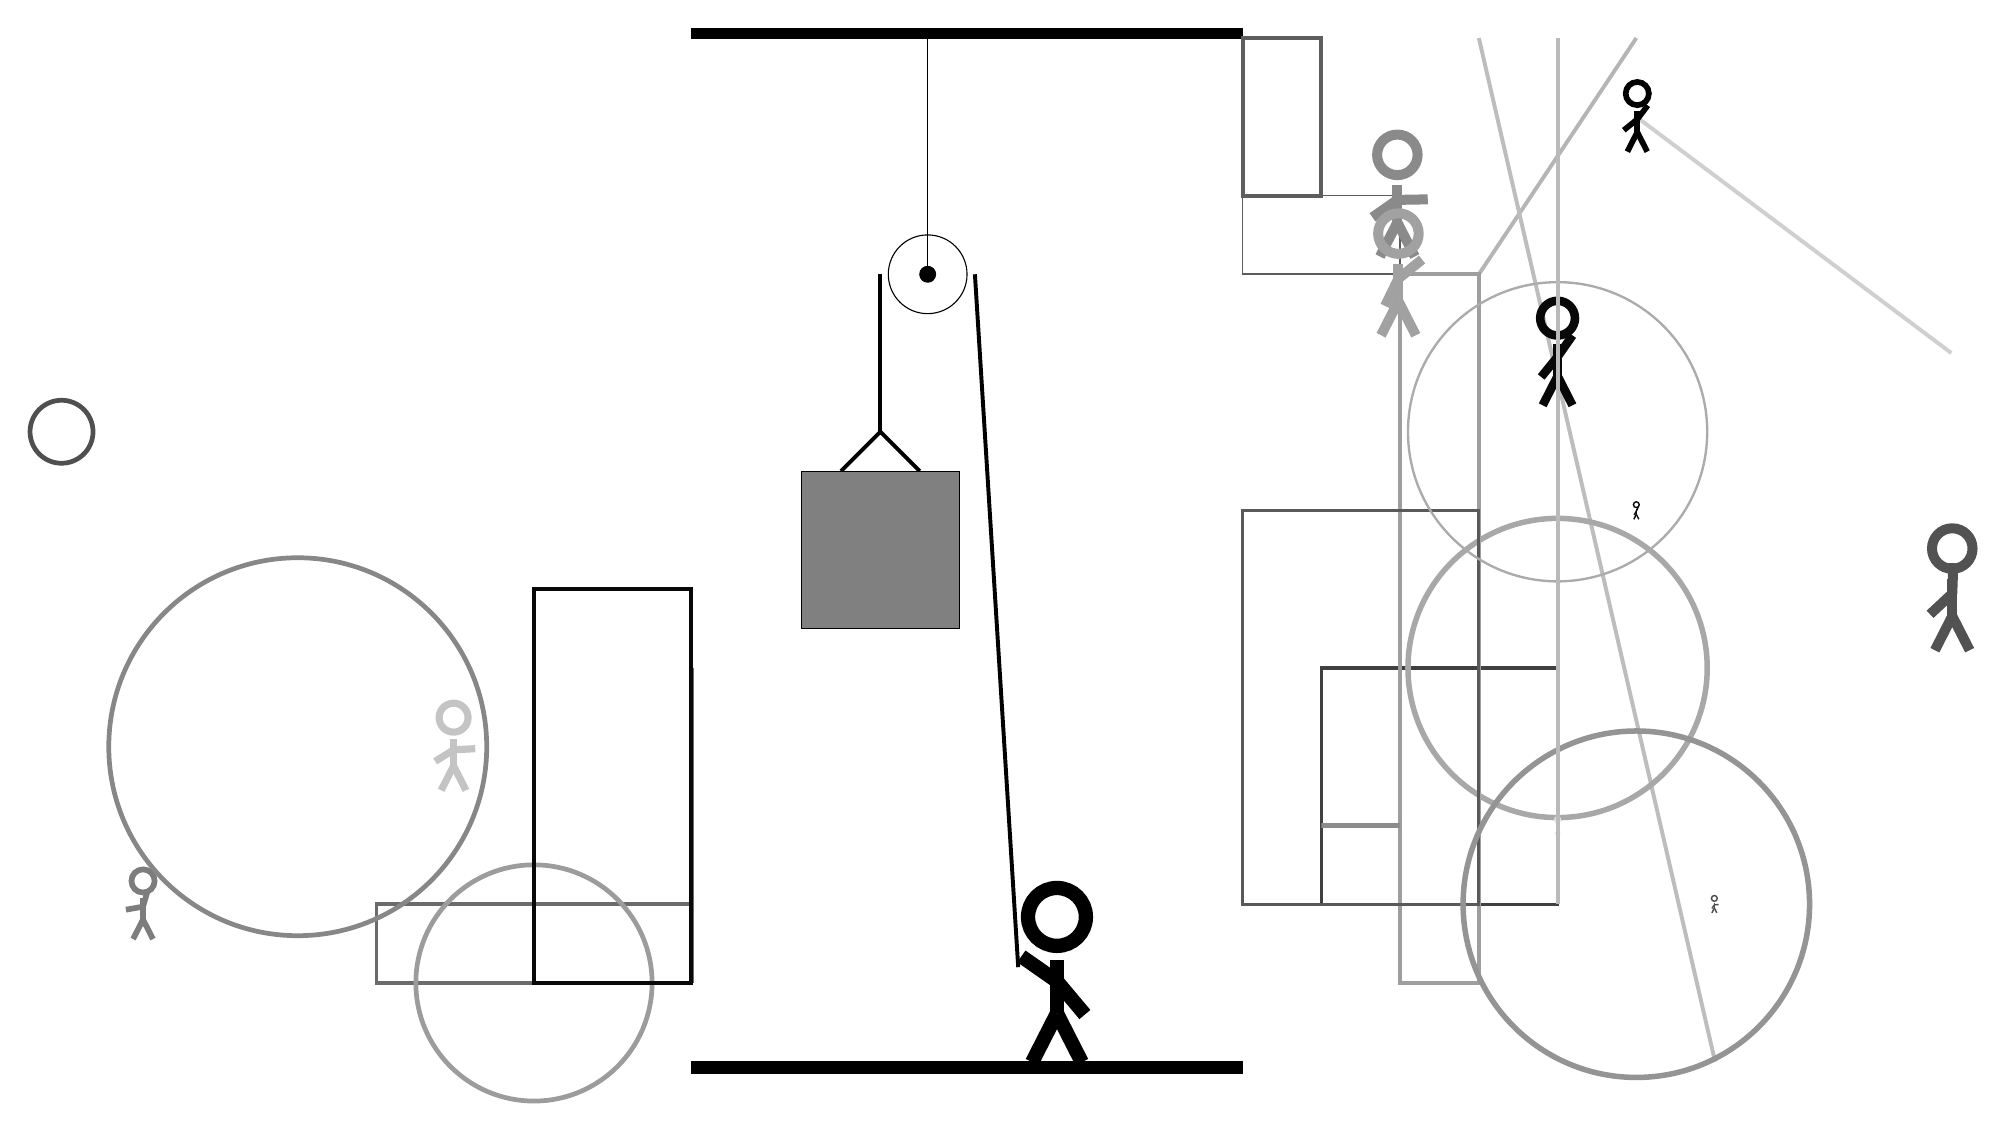
\begin{tikzpicture}
		%%%%% START %%%%%
		
		\draw[fill=black] (-2, 10) rectangle (5, 10.125);
		
		\draw (1, 7) circle (0.5);
		\draw[fill=black] (1, 7) circle (0.1);
		\draw (1, 10) -- (1, 7);
		
		\draw[line width=0.5mm] (-0.1, 4.5) -- (0.4, 5.0) -- (0.9, 4.5);
		\draw[fill=black!50] (-0.6, 4.5) rectangle (1.4, 2.5);
		
		\draw[line width=0.5mm] (0.4, 7) -- (0.4, 5.0);
		\centerarc[line width=0.5mm](1, 7)(0:180:0.6);
		\draw[line width=0.5mm](1.6, 7) -- (2.15, -1.8);
		
		\draw[line width=0.4mm, color=black!75] (6, 2) rectangle (9, -1);
		
		\draw[line width=0.5mm, color=black!58] (-2, -1) rectangle (-6, -2);
		\draw[line width=0.5mm, color=black!29](10, 10) -- (8, 7);
		\draw[line width=0.5mm, color=black!26](8, 10) -- (11, -3);
		\draw[line width=0.5mm, color=black!38] (7, -2) rectangle (8, 7);
		
		\draw[line width=0.7mm, color=black!58] (-2, 2) rectangle (-2, -2);
		
		\draw [line width=0.7mm, color=black!34](9, 2) circle (1.9);
		\node[line width=0.6mm, color=black!68] at (14, 3) {\Strichmaxerl[7][43][88]};
		\draw[line width=0.4mm, color=black!65] (5, 4) rectangle (8, -1);
		\node[line width=0.2mm, color=black!97] at (9, 6) {\Strichmaxerl[6][51][55]};
		\draw[line width=0.5mm, color=black!19](10, 9) -- (14, 6);
		\draw[line width=0.5mm, color=black!63] (6, 8) rectangle (5, 10);
		\draw[line width=0.2mm, color=black!64] (5, 7) rectangle (7, 8);
		
		\draw [line width=0.6mm, color=black!69](-10, 5) circle (0.4);
		\draw [line width=0.6mm, color=black!39](-4, -2) circle (1.5);
		\draw [line width=0.3mm, color=black!33](9, 5) circle (1.9);
		
		\node[line width=0.2mm, color=black!51] at (-9, -1) {\Strichmaxerl[4][10][74]};
		
		\node[line width=0.7mm, color=black!10] at (9, 0) {\Strichmaxerl[1][86][78]};
		\node[line width=0.6mm, color=black!23] at (-5, 1) {\Strichmaxerl[5][32][3]};
		\draw [line width=0.6mm, color=black!47](-7, 1) circle (2.4);
		\draw[line width=0.5mm, color=black!97] (-4, -2) rectangle (-2, 3);
		\node[line width=0.2mm, color=black!46] at (7, 8) {\Strichmaxerl[7][35][1]};
		\node[line width=0.4mm, color=black!69] at (11, -1) {\Strichmaxerl[1][56][3]};
		\node[line width=0.4mm, color=black!100] at (10, 9) {\Strichmaxerl[4][39][53]};
		\node[line width=0.4mm, color=black!37] at (7, 7) {\Strichmaxerl[7][64][39]};
		\draw[line width=0.6mm, color=black!45] (7, 0) rectangle (6, 0);
		
		\draw [line width=0.7mm, color=black!42](10, -1) circle (2.2);
		\node[line width=0.5mm, color=black!96] at (10, 4) {\Strichmaxerl[1][61][65]};
		
		\draw[line width=0.5mm, color=black!27](9, 10) -- (9, -1);
		
		\node at (2.6, -1.9) {\Strichmaxerl[10][-35][-50]};
		
		\draw[fill=black] (-2, -3) rectangle (5, -3.15);
		
		%%%%% END %%%%%
	\end{tikzpicture}
\end{document}